%!TEX root = pfc-memoria.tex
%!TEX encoding = UTF-8 Unicode

\chapter{Manual de instalación}

\epigraph{``Tenemos que dejar de optimizar para programadores y comenzar a optimizar para usuarios.''}{\textsc{Jeff Atwood}}

En este capítulo se describe el procedimiento de instalación de la aplicación y las bibliotecas de las que depende.

\section{Instalación de prerrequisitos}

El primer conjunto de bibliotecas necesarias para instalar son:
\begin{enumerate}
\item El framework de desarrollo \nombrebf{Qt~5.5}
\item El intérprete \nombrebf{Python~3.4}
\end{enumerate}

\subsection{Qt~5.5}

Existen versiones de Qt~5.5 para Mac~OS~X, GNU/Linux y Windows (32 y 64 bit).
En la dirección oficial de descarga para la modalidad de software libre \url{https://www.qt.io/download-open-source/} se puede obtener el fichero de instalación. Se puede realizar una instalación offline u online, pero recomiendo usar el instalador offline ya que necesitamos instalar todos los componentes, incluidos los opcionales.

Proporciona un asistente de instalación de los que estamos acostumbrados, de siguiente-siguiente. Se recomienda usar la carpeta de instalación por defecto en el directorio de casa del usuario, en el caso de Mac~OS~X será \blackdirectory{/Users/USUARIO/Qt5.5.0}. También hace falta marcar la opción de instalación completa, incluido el paquete con el código fuente de Qt, para poder instalar PyQt5.

\begin{figure}[htbp]
\centering
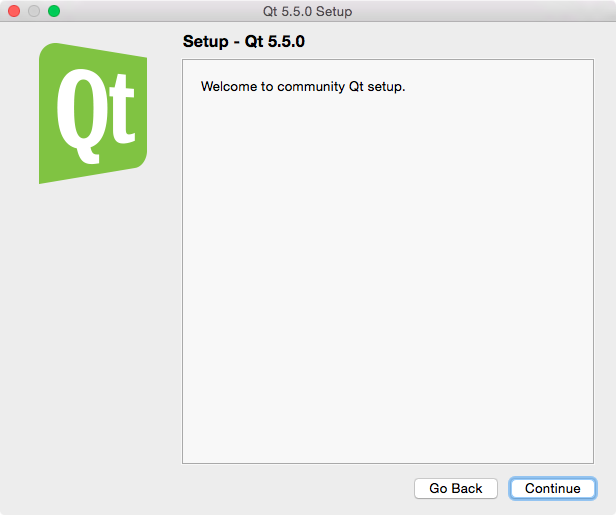
\includegraphics[width=11.5cm]{qt-1}
\caption{Asistente de instalación de Qt~5.5: Página de bienvenida}
\label{fig:qt-1}
\end{figure}

\begin{figure}[htbp]
\centering
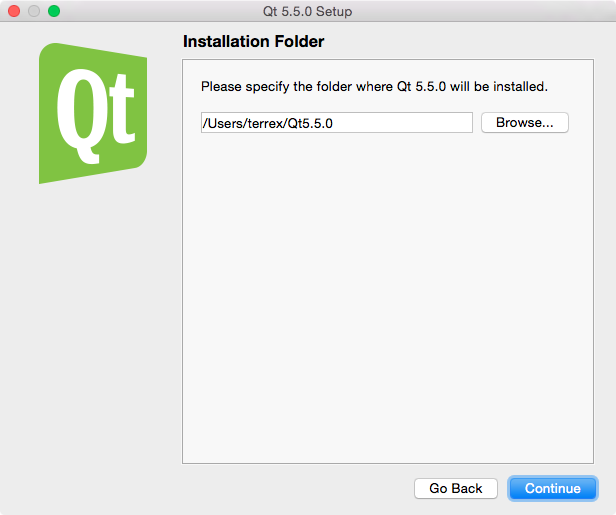
\includegraphics[width=11.5cm]{qt-2}
\caption{Selección de ruta de instalación de Qt}
\label{fig:qt-2}
\end{figure}

\begin{figure}[htbp]
\centering
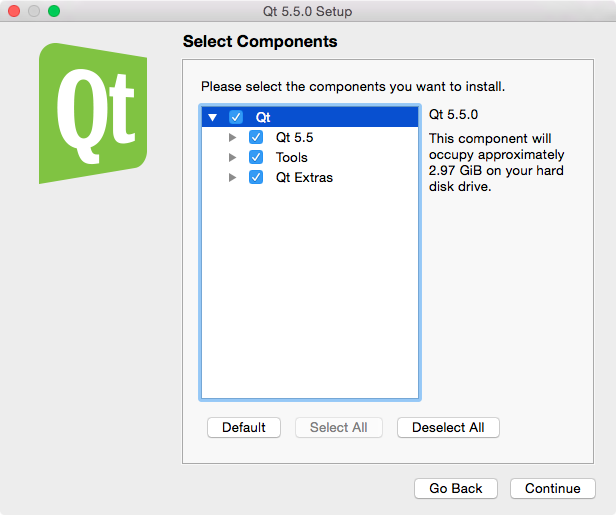
\includegraphics[width=11.5cm]{qt-3}
\caption{Seleccionar todos los componentes para instalar}
\label{fig:qt-3}
\end{figure}

\begin{figure}[htbp]
\centering
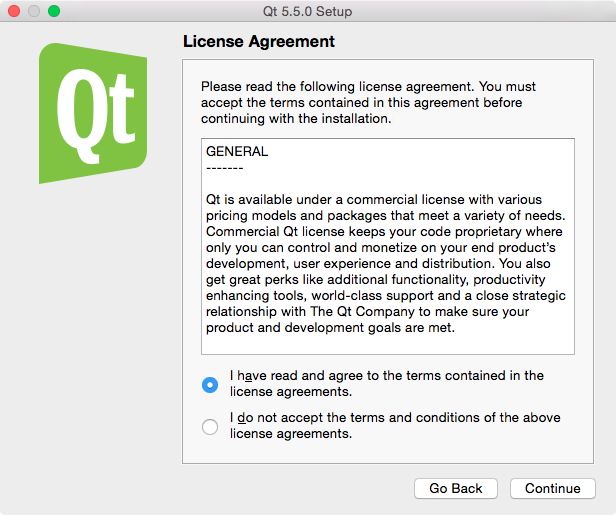
\includegraphics[width=11.5cm]{qt-4}
\caption{Aceptación de licencia}
\label{fig:qt-4}
\end{figure}

\begin{figure}[htbp]
\centering
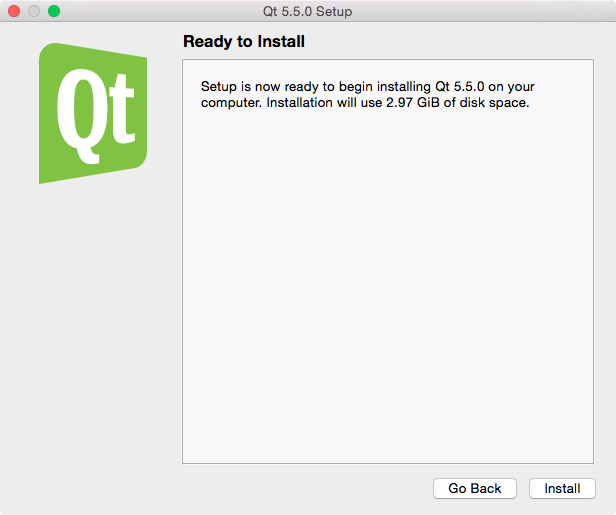
\includegraphics[width=11.5cm]{qt-5}
\caption{Inicio de instalación}
\label{fig:qt-5}
\end{figure}

\begin{figure}[htbp]
\centering
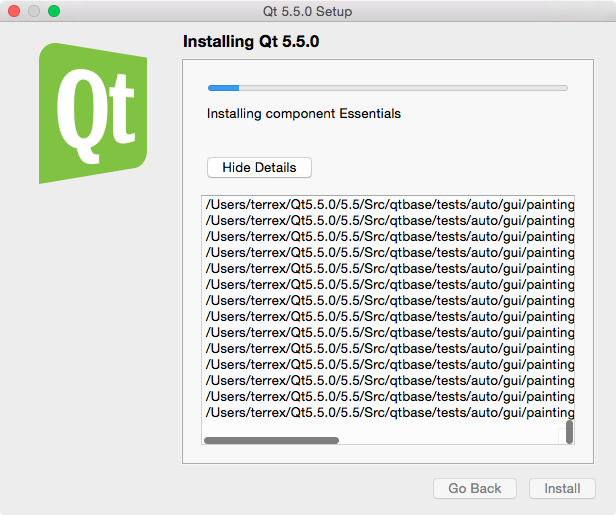
\includegraphics[width=11.5cm]{qt-6}
\caption{Progreso de instalación}
\label{fig:qt-6}
\end{figure}

\begin{figure}[htbp]
\centering
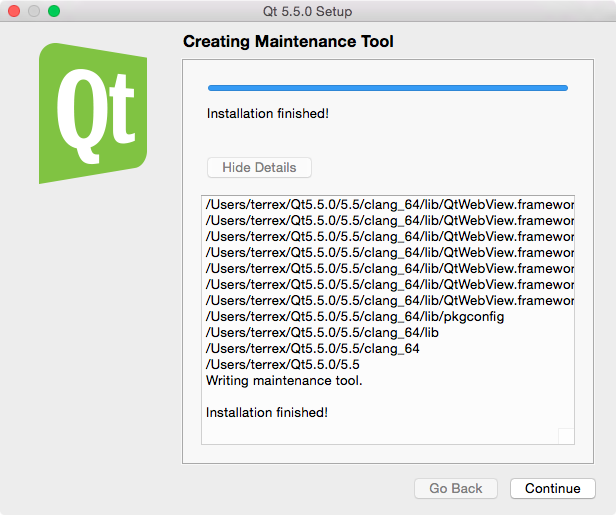
\includegraphics[width=11.5cm]{qt-7}
\caption{Instalación completada}
\label{fig:qt-7}
\end{figure}

\begin{figure}[htbp]
\centering
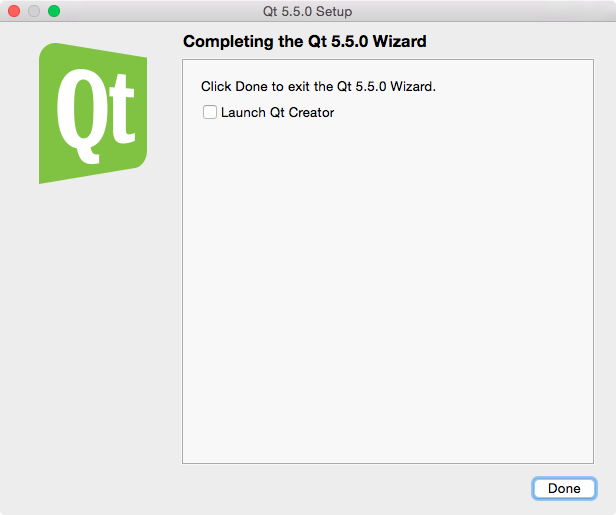
\includegraphics[width=11.5cm]{qt-8}
\caption{Finalización del asistente de instalación de Qt~5.5}
\label{fig:qt-8}
\end{figure}


\subsection{Python~3.4}

Python se encuentra actualmente en dos ``sabores'', versión 2 y versión 3, incompatibles entre sí. En este proyecto nos decantamos por usar el más moderno, y al momento de terminarse el proyecto, la versión concreta que se ha utilizado es Python~3.4.3, aunque debería funcionar en cualquier 3.4.x

Descargar la versión apropiada para su sistema operativo desde la dirección oficial \url{https://www.python.org/downloads/} y seguir las instrucciones del asistente de instalación o de las instrucciones de instalación de la documentación. En el caso de sistemas Mac~OS~X y Windows, se proporciona un asistente de instalación de los binarios; sin embargo para sistemas GNU/Linux se ofrece el paquete del código fuente de Python~3.4.3 listo para compilar.

Otra opción para usar en linux, es utilizar el intérprete Python de su distribución, si es que ésta proporciona alguna versión 3.4, incluyendo el módulo de entornos virtuales \path{venv} y el gestor de paquetes de Python \path{pip} (en Ubuntu son los paquetes \codet{python3-all-dev}, \codet{python3-venv} y \codet{python3-pip}).

\section{Instalación de bibliotecas}

A partir de este momento, tendremos disponibles en la consola el comando de Qt \path{qmake}, y los de Python \path{python3}, \path{pyvenv-3.4} y \path{pip3}.

Es necesario instalar los paquetes de desarrollo. En el caso de Mac~OS~X, la última versión de Xcode; y para Ubuntu, los paquetes listados en el \fullref{lst:ubuntu-apt-get}.

\begin{listing}[htbp]
\begin{minted}{bash}
$ sudo apt-get install ubuntu-dev-tools build-essential \
                       python3-all-dev python3-venv python3-pip \
                       xorg-dev libgl1-mesa-dev libglu1-mesa-dev \
                       libopenblas-dev
\end{minted}
\caption{Paquetes adicionales en Ubuntu}
\label{lst:ubuntu-apt-get}
\end{listing}

\FloatBarrier

Necesitamos las siguientes bibliotecas:
\begin{enumerate}
\item El generador de código \nombrebf{SIP} de Riverbank para la correcta compilación de PyQt5.
\item El \emph{binding} o adaptador de Qt5 para Python llamado \nombrebf{PyQt5} de Riverbank.
\item Los paquetes de pip listados en \blackdirectory{project/requirements.txt}
\end{enumerate}

Los programas de Riverbank pueden descargarse de la página oficial (se pueden probar con versiones futuras sin ningún miedo a perder la compatibilidad hacia atrás):
\begin{itemize}
\item \url{https://riverbankcomputing.com/software/pyqt/download5},\\
archivo \path{PyQt-gpl-5.5.tar.gz}
\item \url{https://www.riverbankcomputing.com/software/sip/download},\\
archivo \path{sip-4.16.9.tar.gz}
\end{itemize}

El primer paso es crear un entorno virtual de Python para evitar conflictos con otras aplicaciones en Python, como paso preventivo, y sin necesidad de tener permisos de superusuario (\autoref{lst:pyvenv}).

\begin{listing}[htbp]
\begin{minted}{bash}
$ pyvenv-3.4 --clear py34
$ source py34/bin/activate
(py34) $ pip3 install -U pip
\end{minted}
\caption[Creación del entorno virtual (pyvenv)]{Creación del entorno virtual (pyvenv), activación y actualización local de \path{pip}}
\label{lst:pyvenv}
\end{listing}
\FloatBarrier

Una vez completado, compilamos e instalamos \path{sip} (\autoref{lst:sip}).

\begin{listing}[htbp]
\begin{minted}{bash}
(py34) $ tar xzf sip-4.16.9.tar.gz
(py34) $ cd sip-4.16.9
(py34) $ python3.4 configure.py
(py34) $ make
(py34) $ make install
(py34) $ cd ..
\end{minted}
\caption{Compilación e instalación de SIP}
\label{lst:sip}
\end{listing}
\FloatBarrier

Después de la instalación de \path{sip}, procedemos a instalar el binding. Nos hemos encontrado un bug en Qt~5.5.0, y necesitamos aplicar un parche previo (\autoref{lst:parche}).

\begin{listing}[htbp]
\begin{minted}{diff}
--- PyQt-gpl-5.5/configure.py   2015-08-07 12:49:40.000000000 +0200
+++ PyQt-gpl-5.5/configure.py   2015-08-07 12:47:23.000000000 +0200
@@ -697,7 +697,7 @@
         lines = f.read().split('\n')
         f.close()
 
-        self.qt_licensee = lines[0]
+        self.qt_licensee = 'Open Source'
         self.qt_shared = (lines[1] == 'shared')
         self.pyqt_disabled_features = lines[2:-1]
 
\end{minted}
\caption[Corrección de bug en Qt~5.5.0]{Corrección de bug en Qt~5.5.0 (\path{PyQt-gpl-5.5-fix-license-typo.diff})}
\label{lst:parche}
\end{listing}
\FloatBarrier

\newpage
Configuramos e instalamos PyQt5 (\autoref{lst:pyqt5}).

\begin{listing}[htbp]
\begin{minted}{bash}
(py34) $ tar xzf PyQt-gpl-5.5.tar.gz
(py34) $ patch -p0 < PyQt-gpl-5.5-fix-license-typo.diff
(py34) $ cd PyQt-gpl-5.5
(py34) $ python3.4 configure.py --qmake ~/Qt5.5.0/5.5/*/bin/qmake
(py34) $ make
(py34) $ make install
(py34) $ cd ..
\end{minted}
\caption{Compilación e instalación de PyQt5}
\label{lst:pyqt5}
\end{listing}
\FloatBarrier

Como último paso, instalamos los paquetes listados como dependencias en el fichero \path{requirements.txt} (\autoref{lst:pip-requirements-txt}).

\begin{listing}[htbp]
\begin{minted}{bash}
(py34) $ pip3 install -r project/requirements.txt
(py34) $ python3.4 -m nltk.downloader all
\end{minted}
\caption{Instalación de paquetes de \codet{pip} de dependencias}.
\label{lst:pip-requirements-txt}
\end{listing}
\FloatBarrier

\section{Inicio del programa}

Para iniciar la ejecución del programa, se puede hacer como se indica en el \autoref{lst:start-pfcsamr}.

\begin{listing}[htbp]
\begin{minted}{bash}
(py34) $ cd project
(py34) $ PYTHONPATH=. pfcsamr/gui.py
\end{minted}
\caption{Inicio del programa}.
\label{lst:start-pfcsamr}
\end{listing}
\FloatBarrier


\chapter{Manual de usuario}

\epigraph{``Los ordenadores son buenos siguiendo instrucciones, no leyendo tu mente.''}{\textsc{Donald Knuth} (1938--)}

\section{Carga del fichero de entrenamiento}

La primera pantalla que se muestra al abrir la aplicación es la pestaña de carga (\autoref{fig:ss-01-load-tab}).

\begin{figure}[H]
\centering
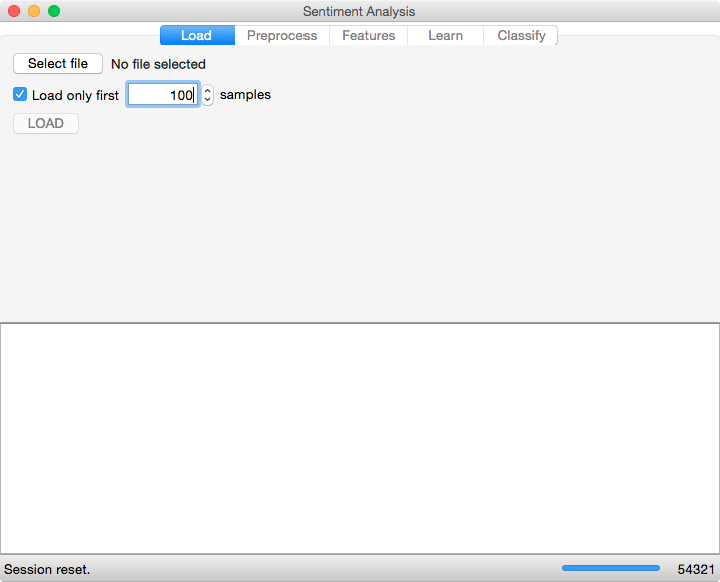
\includegraphics[width=13cm]{ss-01-load-tab}
\caption{Pantalla de carga del fichero de entrenamiento}
\label{fig:ss-01-load-tab}
\end{figure}

\newpage
Al pulsar sobre el botón \menu{Select file} aparece un cuadro de diálogo que permite seleccionar el fichero \path{train.tsv} de entrenamiento (\autoref{fig:ss-02-load-file}).

\begin{figure}[H]
\centering
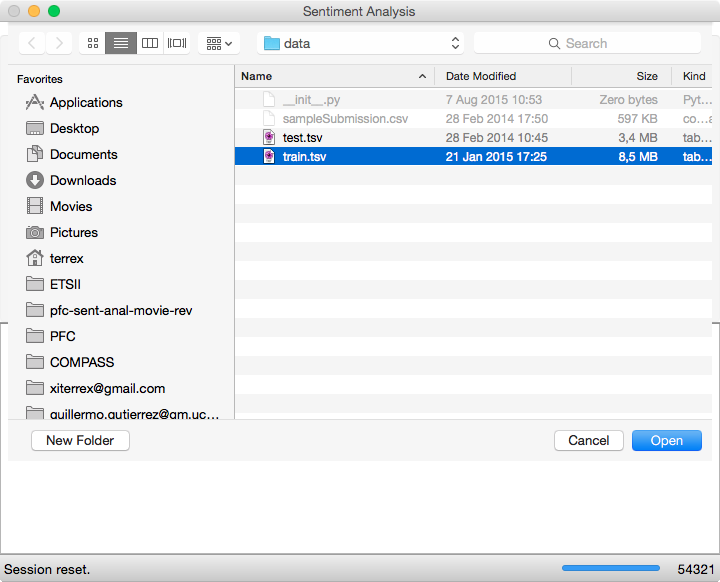
\includegraphics[width=14cm]{ss-02-load-file}
\caption{Pantalla de selección del fichero de entrenamiento}
\label{fig:ss-02-load-file}
\end{figure}

\newpage
Una vez seleccionado, marcar la opción de carga parcial si se desea, indicando el número de muestras. A continuación, pulsar el botón \menu{LOAD}, con lo que aparece el fichero en forma de tabla en el panel de datos (\autoref{fig:ss-03-file-loaded}).

\begin{figure}[H]
\centering
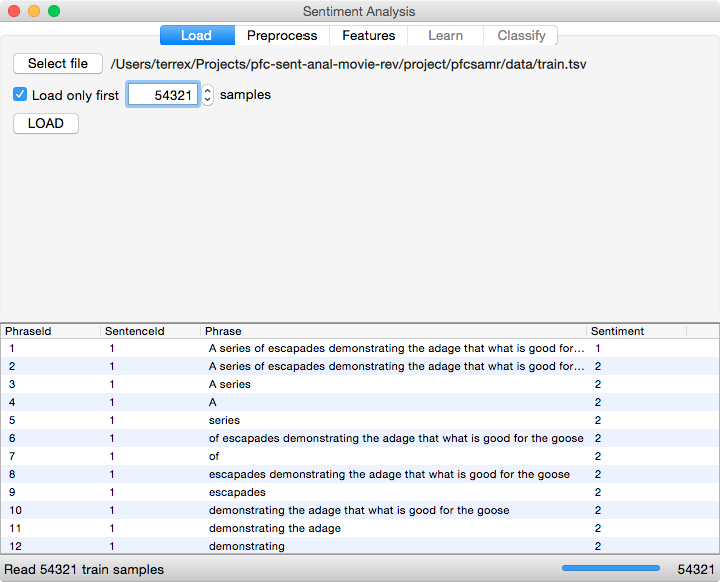
\includegraphics[width=14cm]{ss-03-file-loaded}
\caption{Pantalla con el fichero de entrenamiento cargado}
\label{fig:ss-03-file-loaded}
\end{figure}

\newpage
\section{Opciones de preprocesamiento de texto}
\label{sec:manual-preproc}

Una vez cargado, pasamos a la siguiente pestaña de opciones de preprocesamiento. En esta pantalla, marcamos las opciones deseadas, y a continuación pulsamos el botón \menu{RUN} para proceder al preprocesamiento. Se muestra una barra de progreso a la derecha de la barra de estado, y al terminar, se actualiza el panel de datos con las muestras preprocesadas (\autoref{fig:ss-04-preproc-tab}).

\begin{figure}[H]
\centering
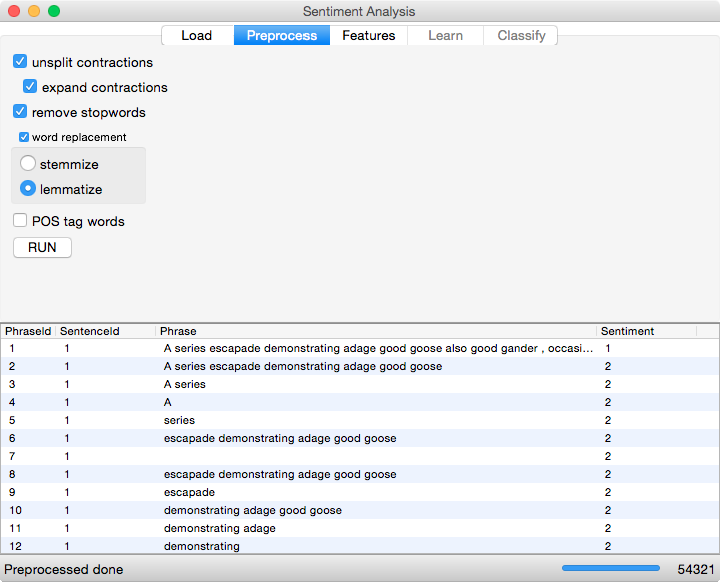
\includegraphics[width=14cm]{ss-04-preproc-tab}
\caption{Pantalla de opciones de preprocesamiento}
\label{fig:ss-04-preproc-tab}
\end{figure}

\newpage
\section{Extracción de características}
\label{sec:manual-features}

El siguiente paso es la extracción de características. Pulsar en la pestaña y marcar las opciones deseadas para la extracción de n-gramas y su reducción. Pulsar en el botón \menu{RUN} para proceder con la transformación. Al finalizar, se muestra el panel de datos con una característica en cada columna, y su valor para cada muestra. El encabezado de la columna indica el n-grama concreto (\autoref{fig:ss-05-feat-tab}).

\begin{figure}[H]
\centering
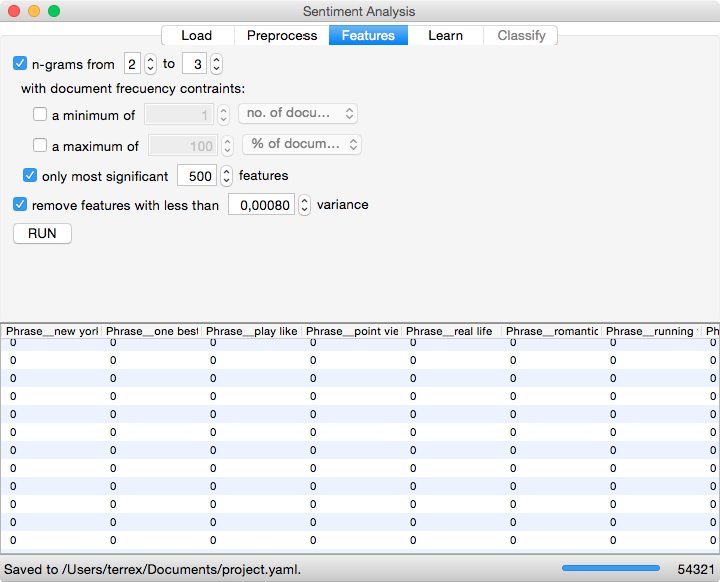
\includegraphics[width=14cm]{ss-05-feat-tab}
\caption{Pantalla de opciones de extracción de características}
\label{fig:ss-05-feat-tab}
\end{figure}

\newpage
\section{Aprendizaje automático del modelo}
\label{sec:manual-learn}

A continuación, avanzamos de pestaña para las opciones de aprendizaje. Se recomienda dejar marcado la división del conjunto en subconjunto de entrenamiento y subconjunto de autoevaluación, para poder obtener una puntuación del modelo aprendido.

Elegir el modelo concreto en la segunda fila de pestañas y pulsar el botón \menu{RUN}. Cuando finalice el aprendizaje, se actualizará el valor de la puntuación (etiqueta \codet{SCORE: }). Hay cinco modelos a elegir, no es obligatorio entrenarlos todos, pero está bien hacerlo para comparar su puntuación y elegir el mejor.

Se puede repetir tantas veces como se desee e ir alterando los parámetros para encontrar la mayor puntuación (\autoref{fig:ss-06-learn-tab}).

\begin{figure}[H]
\centering
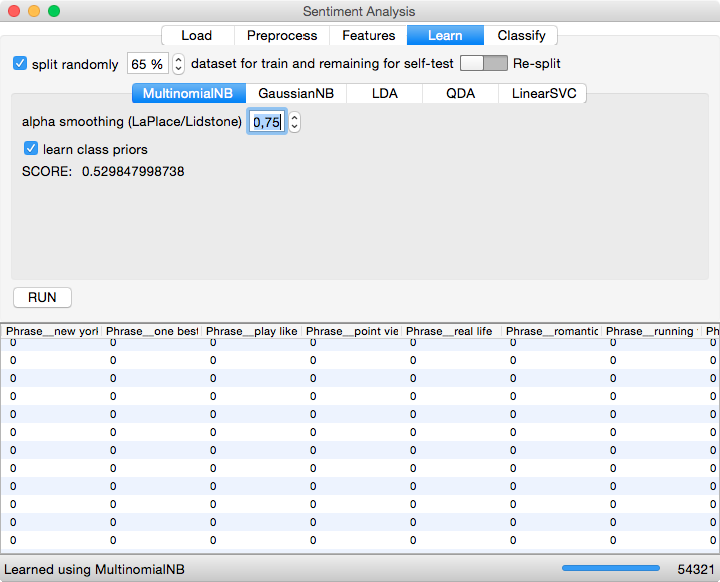
\includegraphics[width=14cm]{ss-06-learn-tab}
\caption{Pantalla de aprendizaje (\codep{MultinomialNB})}
\label{fig:ss-06-learn-tab}
\end{figure}

\newpage
\section{Clasificación del conjunto de clasificación}

Una vez entrenado alguno de los modelos, avanzar pulsando la pestaña siguiente (\autoref{fig:ss-07-classify-tab}). Pulsar el botón \menu{Select file} para elegir el fichero \path{test.tsv} de evaluación.

\begin{figure}[H]
\centering
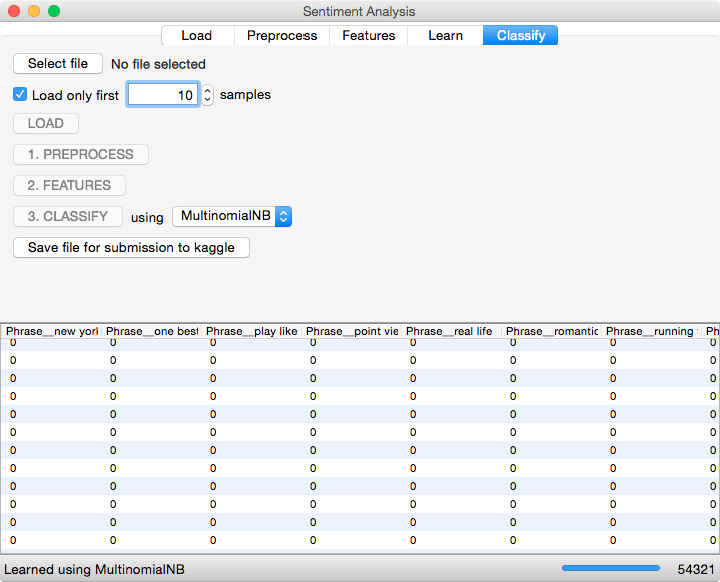
\includegraphics[width=14cm]{ss-07-classify-tab}
\caption{Pantalla de la pestaña de clasificación}
\label{fig:ss-07-classify-tab}
\end{figure}

\newpage
Se puede activar la opción de carga parcial e indicar el número de muestras, si se desea. A continuación pulsar \menu{LOAD} para realizar la carga y la visualización en el panel de datos (\autoref{fig:ss-08-classify-test-loaded}).

\begin{figure}[H]
\centering
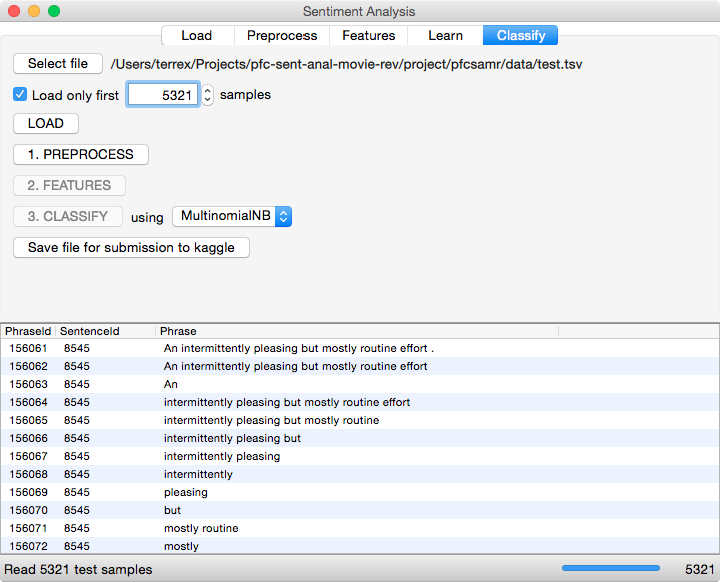
\includegraphics[width=14cm]{ss-08-classify-test-loaded}
\caption{Pantalla con el conjunto de clasificación cargado}
\label{fig:ss-08-classify-test-loaded}
\end{figure}

\newpage
Pulsando el botón \menu{1. PREPROCESS} se realiza el preprocesamiento de texto de clasificación de manera análoga a como se preprocesó el texto de entrenamiento en la fase de entrenamiento (\autoref{sec:manual-preproc}). Se actualizará el panel de datos con el resultado (\autoref{fig:ss-08-classify-test-loaded}).

\begin{figure}[H]
\centering
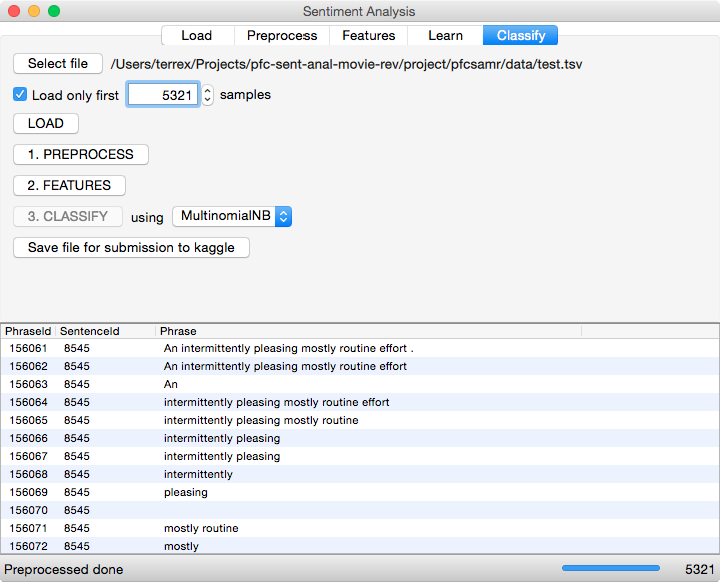
\includegraphics[width=14cm]{ss-09-classify-test-preproccesed}
\caption{Pantalla con el texto preprocesado}
\label{fig:ss-09-classify-test-preproccesed}
\end{figure}

\newpage
Siguiendo con el procedimiento, pulsamos el botón \menu{2. FEATURES} para extraer las características del texto de clasificación preprocesado, que se realiza automáticamente de manera análoga a como se hizo en la fase de entrenamiento (\autoref{sec:manual-features}). Al terminar, se muestra en el panel de datos las características de las muestras a clasificar (\autoref{fig:ss-10-classify-test-featured}).

\begin{figure}[H]
\centering
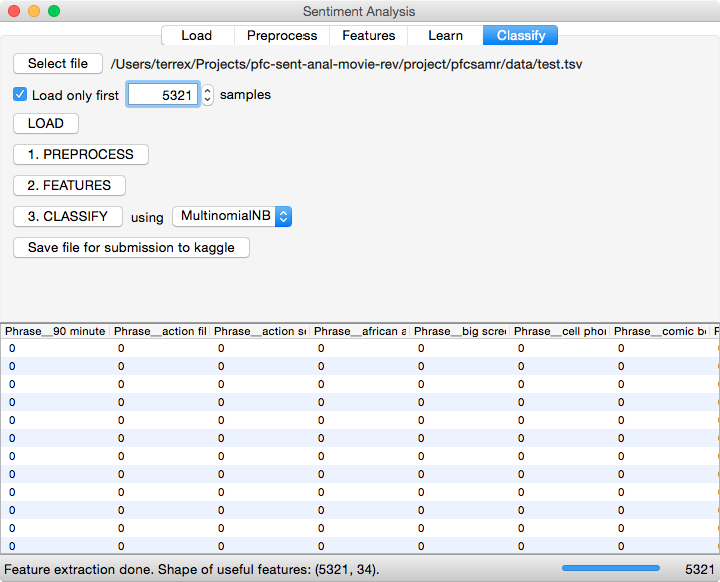
\includegraphics[width=14cm]{ss-10-classify-test-featured}
\caption{Pantalla de características}
\label{fig:ss-10-classify-test-featured}
\end{figure}


\newpage
El último paso es realizar las predicciones. Para ello, elija un modelo del cuadro desplegable. Este modelo debería haber sido entrenado previamente en el paso de entrenamiento (\autoref{sec:manual-learn}), en caso contrario se mostrará un error. Pulsar el botón \menu{3. CLASSIFY} para clasificar las muestras. Aparecerá en el panel de datos las muestras originales con una columna añadida del sentimiento predicho por el modelo seleccionado (\autoref{fig:ss-11-classify-test-predictions}). Si se desea, se puede repetir usando otro modelo.

\begin{figure}[H]
\centering
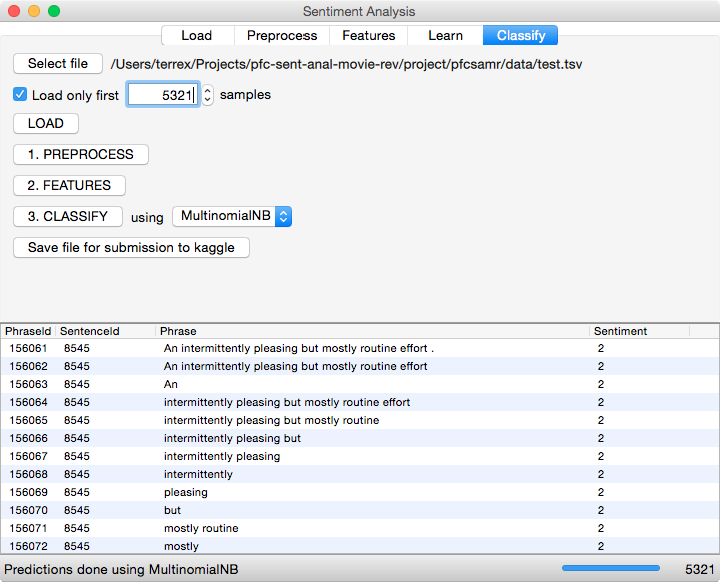
\includegraphics[width=14cm]{ss-11-classify-test-predictions}
\caption{Pantalla con las predicciones de sentimiento}
\label{fig:ss-11-classify-test-predictions}
\end{figure}

Posteriormente, pulsando el botón \menu{Save file for submission to kaggle} se puede guardar el resultado de la clasificación en el formato \path{.csv} para posteriormente entregar en Kaggle.\footnote{\url{https://www.kaggle.com/c/sentiment-analysis-on-movie-reviews}}

\newpage
En cualquier momento, se puede usar el menú \menu{File} para reiniciar el sistema, o abrir o guardar las opciones de la sesión para reanudar posteriormente.

\begin{figure}[H]
\centering
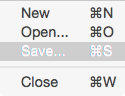
\includegraphics[width=\textwidth]{ss-12-menu-file}
\caption[Pantalla con el menú \codet{FILE}]{Pantalla con el menú \menu{File}}
\label{fig:ss-12-menu-file}
\end{figure}

